\documentclass[draft,ras]{Template/AGUTeX}

\usepackage{graphicx}   % if you want to include graphics files
\usepackage{subfigure}
\usepackage{setspace}
\usepackage{amsxtra}
\usepackage{amsmath}
\usepackage{amssymb}
\usepackage{multirow}
\usepackage{bm}

% graphics path
\graphicspath{{Figs/}}

\authorrunninghead{SWOBODA ET AL.}
\titlerunninghead{3-D ISR}


\authoraddr{Corresponding author: J. P. Swoboda,
Department of Electrical \& Computer Engineering,
Boston University, 8 Saint Mary�s Street
Boston, MA 02215, USA.
(swoboj@bu.edu)}

\begin{document}

\title{Space-Time Ambiguity Function in 3-D ISR}
%%%%%%%%%%%%%% Author Info %%%%%%%%%%%%%%%%%%%%%%%%%%%%%%%%%%%%%
\authors{John Swoboda,\altaffilmark{1}
Joshual Semeter,\altaffilmark{1} Philip Erickson \altaffilmark{2}}

\altaffiltext{1}{Department of Electrical \& Computer Engineering,
Boston University, Boston, Massachusetts, USA.}
\altaffiltext{2}{Atmospheric Science Division,
MIT Haystack Observatory, Westford Massachusetts, USA.}
%%%%%%%%%%%%%% Abstract %%%%%%%%%%%%%%%%%%%%%%%%%%%%%%%%%%%%%

\begin{abstract}By leveraging electronically steerable phased array antenna technology, incoherent scatter radars have now become full three-dimensional remote sensors for ionosphere plasmas. Currently these systems are operating in the high latitude region where the ionosphere is highly dynamic in both space and time. These systems are giving researchers an unprecedented look at the ionosphere that they have not had in the past.

Because of the highly dynamic nature of the ionosphere in this region it is import to differentiate between artifacts and the true behavior of the plasma. Often the three dimension data is fitted in polar coordinates and then the parameters are interpolated to a Cartesian grid. This and other sources of error could be effecting reconstructions of the plasma parameters

In this study we explore the impacts of fast moving plasma progressing through the field of view of the radar on the reconstruction of the three dimensional parameters. We pose the problem as a linear inverse problem for the lags of the plasma autocorrelation function. We will show the impact of the plasma through simulation from a full 3-d incoherent scatter radar model. From there we can apply methods from image and video processing to attempt to correct for the artifacts.
\end{abstract}

%%%%%%%%%%%%%%  End of Abstract %%%%%%%%%%%%%%%%%%%%%%%%%%%%%%%%%%


\begin{article}

%%%%%%%%%%%%%% Intro %%%%%%%%%%%%%%%%%%%%%%%%%%%%%%%%%%%%%

\section{Introduction}
Incoherent scatter radar (ISR) systems have enabled researchers since the 1950's to explore the ionosphere \cite{gordon58}. Using methodology developed by Dougherty, Farley and others these systems can give measurements of electron density $N_e$, Ion temperature $T_i$, electron temperature $T_e$, Ion velocity $V_i$ and other plasma parameters \cite{dougherty:farley1960}, \cite{farleydougherty:ISR2}, \cite{hagfors1961}, \cite{doughteryfarley:ISR3}. These parameters are measured by fitting a theoretic autocorrelation derived from first principles physics to an estimated intrapulse time autocorrelation of the scattered radar signal \cite{Lehtinen1996435}.

As with any real world measurement method there is a non-ideal measurement ambiguity which gives these sensors a type of resolution. Often these ambiguities are only carried out over range and time. The range ambiguity is controlled by the pulse shape and the time ambiguity is controlled by the integration time. A number techniques have been developed to reduce the impact of these ambiguities including full profile analysis \cite{holt1992}. \cite{Lehtinen1989133}, \cite{Lehtinen:1997uh} and deconvolution methods \cite{nikoukar2008}.

Recently phase array technology has started to be leveraged by ISR community. The AMISR systems have already been deployed both at the Poker Flat Alaska and Resolute Bay Canada \cite{amisr.site}. The EISCAT-3D project is currently being developed using phased array technology as well and will be capable of multistaic processing \cite{eiscat3ddesign}. These new systems are already being used to create three dimensional reconstructions of plasma parameters \cite{Semeter2009738}, \cite{Nicolls:2007ie}, \cite{dahlgren2012di},\cite{Dahlgren:2012dq}. 

Even though these systems are already in use there is no formal derivation of a three dimensional ambiguity function for these systems. In a highly dynamic region like the high latitude ionosphere this lack of knowledge can be problematic. There are numerous phenomena such as polar cap patches that may be moving through the field of view at very high speeds \cite{dahlgren2012di}.

These three-dimensional reconstructions often consist of taking the fitted parameters and then interpolating them to a Cartesian space from the system's natural spherical coordinate space \cite{Butler:2013ul}. The step of fitting the autocorrelation function to the theoretical functions to find the final plasma parameters is a non-linear operation. Because of this it is impossible to exactly predict the impact on the parameter values as different plasma populations move through the field of view of the radar. Alternatively it is possible to treat the formation of the autocorrelation estimates as a linear process with each lag as an independent channel \cite{nikoukar2008}.

In this publication we will develop a model for a full three dimensional space-time ambiguity function for 3-D ISR systems. This function can also be modified to show the ambiguity within the rest frame of the moving plasma. In the end this full three dimensional can be represented as kernel in a Fredholm integral equation like in Equation \ref{eqn:friedholm} with $f(s)$ being the lag of the autocorrelation function at a specific time and position. 

\begin{equation}
\label{eqn:friedholm}
g(t) = \int_a^b K(t,s) f(s) ds
\end{equation}

The impact of the three-dimensional ambiguity on moving plasma will be shown through simulation. This ISR simulator fully emulates the ISR data creation process at the IQ level. 

Lastly possible mitigation techniques will be explored. These mitigation techniques will borrow heavily from the image and signal processing literature.


%%%%%%%%%%%%%% Ambiguity Derivation%%%%%%%%%%%%%%%%%%%%%%%%%%%%%%%

\section{Space-Time Ambiguity}

In the ISR literature the measurement ambiguity along the range dimension is often referred to simply as the ambiguity function \cite{hysell2008}. This only shows the measurement ambiguity along the range $r$. Due to the three-dimensional imaging capability of phased array ISR systems we will define a new set of terminology to describe this more complicated measurement which is now imaging the ionosphere in three-dimensional coordinates $\mathbf{r}=[x,y,z]^T$. We will represent the sampled coordinates within the radar with $_s$ such as $\mathbf{r}_s$.

Specifically we will refer to the measurement ambiguity in the range dimension as the range ambiguity, $W(r,r_s,\tau)$. The measurement ambiguity in the elevation and azimuth angles will be referred to as the angular or cross range ambiguity $F(\theta,\phi,\theta_s,\phi_s)$, where $\theta$ is the physical elevation angle, $\phi$ is the physical azimuth angle, $\theta_s$ is the elevation angle that the radar is pointing at and $\phi_s$ is the azimuth angle that the radar is pointing at. The since these two functions are separable they can be multiplied together to form the full spatial ambiguity $K(\tau,\mathbf{r},\mathbf{r}_s)$. Lastly integration time for each measurement will be referred to the time ambiguity. Again like the full spatial ambiguity function we can multiply the space and time ambiguity functions to get the Space-Time ambiguity function which will be represented as $A(\tau,\mathbf{r}_s,\mathbf{r},t_s,t)$.% Might want to go through math from the kernel stuff.

\subsection{Derivation}

In order to develop the space-time ambiguity we will use two different sets of time commonly known in radar literature as fast-time $n$ and slow-time $t$. Fast-time looks at time on the order of the radar systems A/D conversion while slow-time time is looking at time on the order of the system's pulse repetition interval \cite{richards:fundamentalsigproc}. We will use the same reference for fast-time but slow time will be the time it takes the plasma to change state and thus change the ACF.

In order to start we will first develop the range ambiguity which is due to the pulse shape and receiver filter on the ISR systems. If we look at data received by the ISR system at time $n$, with a wavenumber $\mathbf{k}$ and pulse shape $s(n)$, noted as $x(n)$ we can see that the received signal can be represented as the following

\begin{equation}
\label{eq:xt}
x(n) \propto h(n) \ast \int_{\mathbf{r}} e^{-j\mathbf{k} \cdot \mathbf{r}}  s(n-\frac{2r}{c}) n_e(\mathbf{r},n) d\mathbf{r},
\end{equation}

\noindent where $h(n)$ is the receiver filter, $n_e(\mathbf{r},n)$ is the electron density fluctuation.  Generally it is assumed that the pass band of the filter is larger then the bandwidth of the electron density fluctuation \cite{kudeki:notes}.  As such it can  be assumed that filter will only act on the the shape of the pulse.   This will change Equation \ref{eq:xt} to the following:

\begin{equation}
\label{ex:xtaug}
x(n) \propto \ast \int_{\mathbf{r}} e^{-j\mathbf{k} \cdot \mathbf{r}}  a(n-\frac{2r}{c}) n_e(\mathbf{r},n) d\mathbf{r}
\end{equation}
\noindent where $a(n)= h(n) \ast s(n)$.   

When the autocorrelation of the signal is done we find the following formula, \cite{nikoukar2008}.  

\begin{equation}
\label{ex:acf1}
\langle x(n)x^*(n+\tau)\rangle = \int_{\mathbf{r'}}\int_{\mathbf{r}} e^{-2j \mathbf{k}\cdot \left(\mathbf{r}'-\mathbf{r} \right)}a(n-\frac{2r}{c})a^*(n+\tau-\frac{2r'}{c}) \langle n_e(\mathbf{r},n)n_e(\mathbf{r}',n+\tau)\rangle d\mathbf{r} d\mathbf{r}'
\end{equation}
 
\noindent where $r'$ is the magnitude of the vector $\mathbf{r}'$. We can make some simplifying assumption at this point that the space-time autocorrelation function of $n_e(\mathbf{r},t)$, $\langle n_e(\mathbf{r},n)n_e(\mathbf{r}',n+\tau)\rangle$, will vanish as the magnitude of $\mathbf{x} \equiv \mathbf{r}'-\mathbf{r} $ increases.  Once the spatial correlation is removed we can rewrite Equation \ref{ex:acf1} as 
 
 \begin{equation}
 \label{ex:acf2}
 \langle x(n)x^*(n+\tau)\rangle = \int_{\mathbf{r}} a(n-\frac{2r}{c})a^*(n+\tau -\frac{2r}{c}) \int_{\mathbf{x}} e^{-2j \mathbf{k}\cdot \mathbf{x}} \langle n_e(\mathbf{r},n)n_e(\mathbf{x}+\mathbf{r},n+\tau)\rangle d\mathbf{x} d\mathbf{r}.
 \end{equation}
 
 The inner integral is a spatial Fourier transform evaluated at the wave number of the radar $\mathbf{k}$
 \begin{equation}
 \label{eq:spft}
 \langle |n_e(\mathbf{k},r,\tau)|^2\rangle \equiv  \int_{\mathbf{x}} e^{-2j \mathbf{k}\cdot \mathbf{x} } \langle n_e(\mathbf{r},b)n_e(\mathbf{x}+\mathbf{r},n+\tau)\rangle d\mathbf{x}.
 \end{equation}
 
 \noindent Equation \ref{ex:acf2} becomes
 
 \begin{equation}
 \langle x(n)x^*(n+\tau)\rangle = \int_{r} a(n-\frac{2r}{c})a^*(n+\tau -\frac{2r}{c}) \langle |n_e(\tau,\mathbf{k},\mathbf{r})|^2\rangle dr.
 \end{equation}
 %angle ambiguity
 %E_e(\phi,\psi)\text{dirc}_N(\frac{d_1}{\lambda}\sin\phi \cos\psi)\text{dirc}_K\left(\frac{d_2}{\lambda}\sin\phi\sin\psi\right)
 It should be noted that the term $ a(n)a^*(n+\tau)$ is the soft target ambiguity function.  If $n$ is replaced with $2r_s/c$ we can see that the this function represented as $W(\tau,r_s,r)$ \cite{nikoukar:thesis}.  In order to simplify notation we will represent $ \langle |n_e(\tau,\mathbf{k},\mathbf{r})|^2\rangle$, as $R(\tau,\mathbf{r})$. Assuming, for the moment, that $R$ only varies across the range dimension $r$ we can now represent this in the form of a Fredholm integral equation
 
 \begin{equation}
 \label{eqn:fredfirst}
 \langle x(2r_s/c)x^*(2r_s/c+\tau)\rangle = \int_{r} W(\tau,r_s,r) R(\tau,r) dr.
 \end{equation}
 
This function is in a way a lag dependent smoothing along the range dimension of $R(\tau,r)$. 
 
The spatial ambiguity across angle is determined by the antenna beam pattern. In phase array radars this beam pattern is ideally the array factor multiplied by the element pattern \cite{Balanis:2005:ATA:1208379}. The array factor is determined by a number of things including the element spacing in both x and y $(dx,dy)$ and the wave number of the radar, $k$. Making idealized assumptions with no mutual coupling and that the array elements are cross dipole elements AMISR systems will have the following array pattern for pointing angle ($\theta_s,\phi_s$),
 
 \begin{equation}
 \label{eqn:amisrpat}
F(\theta,\phi,\theta_s,\phi_s) = \frac{1}{2}(1+\cos(\theta)^2)\left[ \frac{1}{MN} \left(1+e^{j(\psi_y/2 + \psi_x)}\right)\frac{\sin((M/2) \psi_x)}{\sin(\psi_x)} \frac{\sin((N/2) \psi_x)}{\sin(\psi_x/2)}\right]^2,
 \end{equation}
 
 \noindent where $\psi_x = -k d_x(\sin\theta\cos\phi-\sin\theta_s\cos\phi_s)$, $\psi_y = -k d_y(\sin\theta\sin\phi-\sin\theta_s\sin\phi_s)$.


This spatial ambiguity is a separable function made up of the components of $W(\tau,r)$ and $F(\theta,\phi,\theta_s,\phi_s)$. These two functions can be combined by multiplying, creating the spatial ambiguity function  $K(\tau,\mathbf{r}_s,\mathbf{r})$, and then doing a volume integration. This will create radar system's estimate of the ACF which will be referred to as $\rho(\tau,\mathbf{r}_s)$,

 %\begin{equation}

 \begin{align}
  \label{eqn:volume}
\rho(\tau,\mathbf{r}_s) &= \int F(\theta,\phi,\theta_s,\phi_s)W(\tau,r_s,r) R(\tau,\mathbf{r}) dV,\\
	&= \int K(\tau,\mathbf{r}_s,\mathbf{r}) R(\tau,\mathbf{r})dV.
\end{align}
 %\end{equation}

A rendering of an example of this full ambiguity function for an uncoded long pulse and antenna pattern in (\ref{eqn:amisrpat}) for four beams can be seen in Figure \ref{fig:amb4}.

\begin{figure}
	\centering
	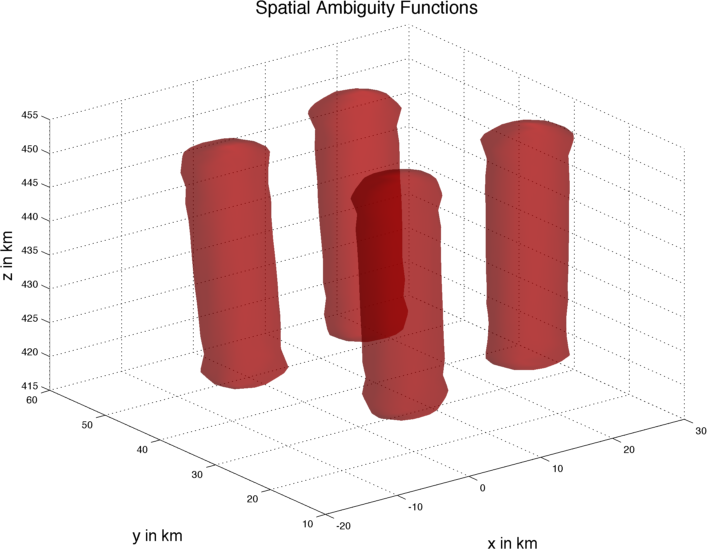
\includegraphics[width=5.5in]{spaceamb}
	\caption{Full Spatial Ambiguity Function}	
	\label{fig:amb4}
\end{figure}

Lastly, since the radar requires a finite amount of time to average pulses to create the estimate of the ACF we will add slow-time dependence to $R$. We will add another separable function $G(t_s,t)$ to the kernel,


\begin{align}
\label{eqn:sptamb}
\rho(\tau,\mathbf{r}_s,t_s) &= \int G(t_s,t)K(\tau,\mathbf{r}_s,\mathbf{r})R(\tau,\mathbf{r},t) dV dt\\
	&=\int L(\tau,\mathbf{r}_s,t_s,\mathbf{r},t)R(\tau,\mathbf{r},t)d\mathbf{r}dt.
\end{align}

\noindent The final kernel, $L(\tau,\mathbf{r}_s,t_s,\mathbf{r},t)$ encompasses the full space-time ambiguity.

\subsection{Ambiguity after Frame Transformation}

We will now focus on the impact of the motion of plasma as it is going through the field of view of the radar. We will assume that the radar is integrating over a length of time $T$ beginning at $t_s$. The kernel $L$ will be represented as a separable function $K$ and $G$ as in (\ref{eqn:sptamb}). In this case $G$ will be an indicator function of length $T$ and centered at $t_0+1/2$. This will change (\ref{eqn:sptamb}) to the following,

\begin{equation}
\label{eqn:L2}
\rho(\tau,\mathbf{r}_s,t_s) = \int K(\tau,\mathbf{r}_s,\mathbf{r}) \int_{t_s}^{t_s+T}R(\tau,\mathbf{r},t) dt dV.
\end{equation}

At this point it will be assumed that the plasma is rigid object and will not deform with respect to $\mathbf{r}$ over time period $[t_0,t_0+T]$. Also it will be assumed that it will be moving with a constant velocity $\mathbf{v}$. Thus $R(\tau,\mathbf{r},t)\Rightarrow R(\tau,\mathbf{r}+\mathbf{v}t)$. At this point (\ref{eqn:L2}) becomes,

\begin{equation}
\label{eqn:L3}
\rho(\tau,\mathbf{r}_s,t_s) = \int \int_{t_s}^{t_s+T} K(\tau,\mathbf{r}_s,\mathbf{r})R(\tau,\mathbf{r}+\mathbf{v}t)dtdV\end{equation}

A change of variables where $\mathbf{r}' = \mathbf{r}+\mathbf{v}t$ acts as a Galilean transform and applies a warping to the kernel and changing the frame of reference. Then (\ref{eqn:L3}) becomes

\begin{equation}
\label{eqn:L4}
\rho(\tau,\mathbf{r}_s,t_s)= \int \int_{t_0}^{t_0+T} K(\tau,\mathbf{r}_s,\mathbf{r}'-\mathbf{v}t)R(\tau,\mathbf{r}')dtdV.
\end{equation}

\noindent Since $R(\tau,\mathbf{r}')$ is no longer dependent on $t$ (\ref{eqn:L4}) becomes,

\begin{equation}
\label{eqn:L5}
\rho(\tau,\mathbf{r}_s,t_s)= \int \left[ \int_{t_0}^{t_0+T}  K(\tau,\mathbf{r}_s,\mathbf{r}'-\mathbf{v}t)dt \right]R(\tau,\mathbf{r}+\mathbf{v}t)dV.
\end{equation}

By performing the integration in $t$ the problem can now be simplified further back to a Fredholm integral equation by simply replacing the terms  in the square brackets as a new kernel $A$,

\begin{equation}
\label{eqn:L6}
\rho(\tau,\mathbf{r}_s,t_s)= \int A(\tau,\mathbf{r}_s,t_s,\mathbf{r}') x_i(\mathbf{r}')dV.
\end{equation}

\noindent The impact of the plasma velocity on the ambiguity function can be seen in Figure \ref{fig:ambtime}. This is the same ambiguity as seen in \ref{fig:amb4} but with a velocity of $100$ m/s in the $y$ direction. This distortion shows in the spatial domain that the motion of the plasma creates a larger ambiguity function in space and thus blurs the image further.

\begin{figure}[!t]
	\centering
	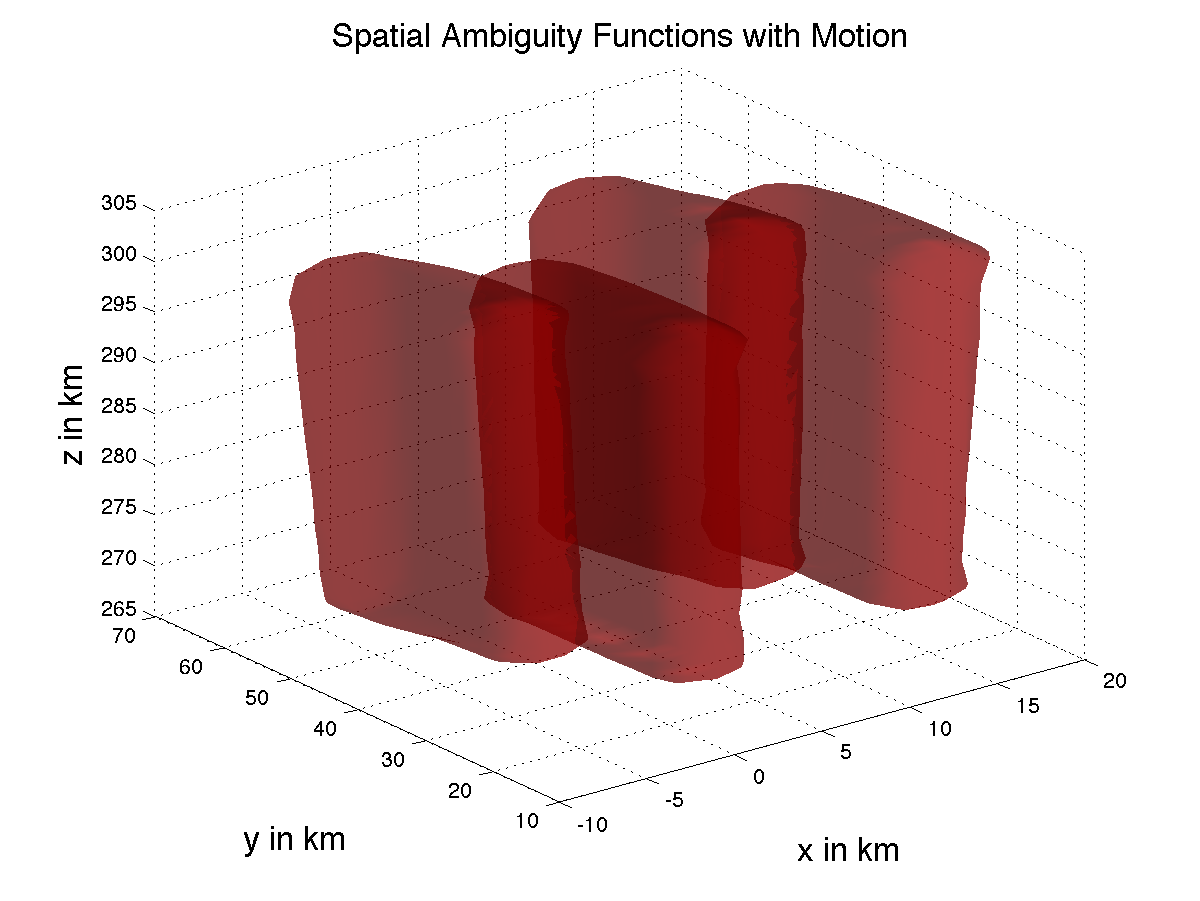
\includegraphics[width=5.5in]{spaceambmoving}
	\caption{Full Spatial Ambiguity Function With Motion}
	\label{fig:ambtime}
\end{figure}

The operator $A$ can be estimated through knowledge of the radar system and pulse pattern which would determine the antenna beam pattern and the range ambiguity function. The velocity $\mathbf{v}$ can be estimated by taking taking measurements of the Doppler shift and using a methodology seen in \cite{butler:imagingfregiondrifts}. Once the operator has been determined debluring methods can be applied.

%%%%%%%%%%%%%% Simulation %%%%%%%%%%%%%%%%%%%%%%%%%%%%%%%%%%%%%

\section{Simulation}

In order to determine if it is possible to improve the resolution of ISR processing synthetic data was created using a known condition of a simulated ionosphere. The simulator creates data by deriving filters from the autocorrelation function and applying it to complex white Gaussian noise. In a sense every point in time and space noise plant and filter structure as in Figure \ref{fig:IQdiagram}. The data is then scaled and summed together according to its location in range and angle space to radar.

\begin{figure}[h!]
\centering
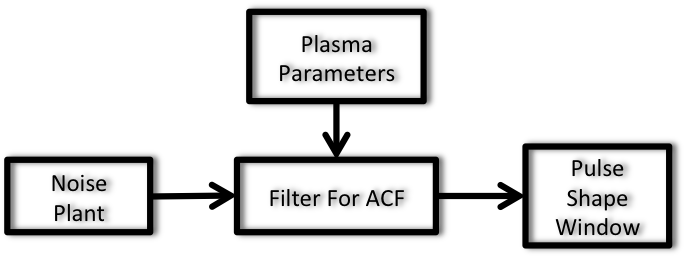
\includegraphics[width=3in]{diagrampart}
\caption{I/Q Simulator Diagram}
\label{fig:IQdiagram}
\end{figure}

To test this a phantom ionosphere is created where a small plasma enhancement moves through the radar field of view. The background electron density varies in altitude as a Chapman function while the electron and ion temperature remains constant. This is done to avoid having to do full fit and thus only try to measure the electron density. Also estimates of the zeroth lag are only necessary. Added to this is a 35 km radius sphere of enhance electron density of about $5\times 10^{10} $ m$^{-3}$ centered at 400 km altitude moving at 500 m/s along the y direction.

%%%%%%%%%%%%%% Mitigation %%%%%%%%%%%%%%%%%%%%%%%%%%%%%%%%%%%%%

\section{Possible Mitigation Techniques}
%%%%%%%%%%%%%% Conclusion %%%%%%%%%%%%%%%%%%%%%%%%%%%%%%%%%%%%

\section{Conclusion}
\bibliographystyle{BibTeX/agufull08}
\bibliography{BibTeX/litreview}

\begin{acknowledgments}
(Text here)
\end{acknowledgments}

\end{article}

\end{document}